\documentclass[]{scrartcl}
\title{Vorlesung Analysis II}
\usepackage{amsmath,amssymb,amsfonts}
\usepackage{stmaryrd}
\usepackage{mathtools}
\usepackage{latexsym}
\usepackage{graphicx}
\usepackage{tikz}
\usepackage{xcolor}
\usepackage[most]{tcolorbox}
\usepackage{soul}
\usepackage{ upgreek }
\usepackage{hyperref}
\usepackage{tipa}
\usepackage[dvipsnames]{xcolor}
\hypersetup{
	colorlinks=true,
	linkcolor=blue,
	filecolor=magenta,      
	urlcolor=cyan,
	pdftitle={Overleaf Example},
	pdfpagemode=FullScreen,
}
\newcommand{\redcircle}[1]{%
	\tikz[baseline=(char.base)]{
		\node[shape=circle, draw=red, text=red, thick, inner sep=1pt] (char) 
		{\textbf{#1}};
	}%
}
\newcommand{\bluecircle}[1]{%
	\tikz[baseline=(char.base)]{
		\node[shape=circle, draw=blue, text=blue, thick, inner sep=1pt] (char) 
		{\textbf{#1}};
	}%
}
\newcommand{\blackcircle}[1]{%
	\tikz[baseline=(char.base)]{
		\node[shape=circle, draw=black, text=black, thick, inner sep=1pt] 
		(char) 
		{\textbf{#1}};
	}%
}
\newcommand{\orangecircle}[1]{%
	\tikz[baseline=(char.base)]{
		\node[shape=circle, draw=orange, text=orange, thick, inner sep=1pt] 
		(char) 
		{\textbf{#1}};
	}%
}
\newcommand{\redul}[1]{\setulcolor{red}{\ul{#1}}}
\newcommand{\blueul}[1]{\setulcolor{blue}{\ul{#1}}}
\newcommand{\yelul}[1]{\setulcolor{yellow}{\ul{#1}}}
\newcommand{\greenul}[1]{\setulcolor{green}{\ul{#1}}}
\newcommand{\oraul}[1]{\setulcolor{orange}{\ul{#1}}}
\setul{1pt}{3pt} % Linienhöhe und Abstand zum Text (optional anpassbar)

\setlength{\topmargin}{-.5in} \setlength{\textheight}{9.25in}
\setlength{\oddsidemargin}{0in} \setlength{\textwidth}{6.8in}
\setlength{\parindent}{0pt}

\begin{document}
	\maketitle
	\textbf{\underline{Teil 3: Gewöhnliche Differentialgleichungen}}\\
	\\
	\textbf{\underline{an21: Lineare DGLn n-ter Ordnung mit Konstanten Koeffizienten}}\\
	\\
	\textbf{\underline{\underline{Stichworte:} Linearität der Lösungsmenge, $\phi$=charakteristisches Polynom, Operatormethode, D = Differntialoperator, r.S. = rechte Seite, l.S. = linke Seite}}\\
	\\
	\textbf{\underline{Literatur:}} \blueul{[Hoffmann]: Kapitel 7.8., [Heuser]: Kapitel 16}\\
	\\
	\textbf{21.1. \underline{Einleitung:}} Behandeln mit der Operatormethode Lineare DGLn n-ter Ordnung mit Konstanten Koeffizienten, homogen und inhomogen. Speziell den Fall n=2.\\
	\\
	\textbf{21.2. \underline{Vereinbarung:}} Betrachten für $n\in \mathbb{N}$ fest, $a_0,...,a_{n-1} \in \mathbb{R}, f:j\rightarrow\mathbb{K},$ \redul{$\mathbb{K}\in\{\mathbb{R},\mathbb{C}\}$}, \\
	Die DGL \fcolorbox{red}{white}{$u^{(n)}+a_{n-1}u^{(n-1)}+...+a_1u'+a_0u=f$} $\blackcircle{*}$\\
	\\
	\textbf{21.3. \underline{Motivation:}} Haben schon n=1 behandelt, daneben ist n=2 wichtig.\\
	\\
	\textbf{21.4. \underline{Def.:}} Für $f\neq0$ heißt $\blackcircle{*}$ eine \redul{inhomogene Lineare DGL n-ter Ordnung mit Konstanten Koeffizienten,} f heißt \redul{Inhomogenität} oder \redul{Störglied}.\\
	Die zugehörige \underline{homogene} DGL (linear, n-ter Ordnung, mit Konstanten Koeffizienten) lautet $\blackcircle{*}_h$ \fcolorbox{red}{white}{$u^{(n)}+a_{n-1}u^{(n-1)}+...+a_1u'+a_0u=0$}.\\
	\\
	\textbf{21.5. \underline{Linearitätsüberlegungen:}} (a) \greenul{u,v Lsgn.} von $\blackcircle{*}_h \Rightarrow \forall\alpha, \beta \in \mathbb{K}:$ \greenul{$\alpha u+\beta v$ Lsg.} von $\blackcircle{*}$, d.h. doie Menge der Lösungen der homogenen DGL $\blackcircle{*}_h$ liefert einen \greenul{Vektorraum}.\\
	(b) \greenul{u Lsg.} von $\blackcircle{*} \wedge$ \greenul{v Lsg.} von \greenul{$\blackcircle{*}_h$} $\Rightarrow$ \greenul{u+v Lsg.} von $\blackcircle{*}$\\
	(c) \greenul{v,w Lsgn.} von $\blackcircle{*}$ $\Rightarrow$ \greenul{v-w Lsg. von $\blackcircle{*}_h$}\\
	(d) Ist y=u+iv mit u,v:j $\rightarrow \mathbb{R}, i=\sqrt{-1},$ so gilt:\\
	\greenul{y (Komplexe) Lsg. von $\blackcircle{*}$} $\Leftrightarrow$ \greenul{u,v (reelle) Lsgn. von $\blackcircle{*}$} mit \greenul{Re$ f, Ym f$ als r.l.}\\
	\\
	\underline{Bem.:} Alle Lsgn. von $\blackcircle{*}$ erhält man durch Addition irgendeiner \redul{spzillen (partikulären) Lsg.}  zu einer (beliebigen) von $\blackcircle{*}_h$.\\
	\\
	\textbf{21.6. \underline{Def.:}} Das zu $\blackcircle{*}$ gehörige Polynom \yelul{$\phi(\lambda)$}$:=\lambda^n+a_{n-1}\lambda^{n-1}+...+a_1\lambda+a_0, \lambda\in\mathbb{K}$,\\
	Heißt das \redul{charaktistische Polynom} von $\blackcircle{*}$,\\
	Die Gleichung $\phi(\lambda)=0$ heißt \redul{charakteristische Glg.}\\
	\\
	\textbf{21.7. \underline{Spezialfall \underline{n=2:}}} $\blackcircle{*}:u''+au'+bu=f, \blackcircle{*}_h: u''+au'+bu=0,$\\
	wo a,b $\in \mathbb{R}, f:j\rightarrow\mathbb{K}$ stetig.\\
	Das charakteristische Polynom ist $\phi(\lambda)=\lambda^2+a\lambda+b, \lambda\in\mathbb{K}$\\
	und $\lambda^2+a\lambda+b=0$ ist die charakteristische Glg.\\
	\\
	\textbf{21.8. \underline{Def.:}} Der \redul{Ableitungsoperator D} seei definiert durch \yelul{Du:=u'} für u:j$\rightarrow\mathbb{K}$ bel. oft diff'bar.\\
	\\
	\textbf{21.9. \underline{Bem.:}} D:$\phi^{\infty}(j,\mathbb{K})\rightarrow\phi^\infty(j,\mathbb{K})$ \greenul{ist Linear}.\\
	\\
	\textbf{21.10. \underline{Def.:}} Mit \yelul{$D^0=E$}:=$id_{\phi^\infty(j,\mathbb{K})}$ und \yelul{$D^{k+1}$}:=$DD^k, k\in \mathbb{N}_0,$ sind bel. Potenzen und Linearkombinationen davon definiert.\\
	\\
	\textbf{21.11. \underline{Bem.:}} $\bullet$ Haben \greenul{Eu=u, $D^ku=u^{(k)}$}, für $k\in \phi^\infty(j,\mathbb{K}).$\\
	$\bullet$ Haben die \redul{Verauschbarkeitsbeziehung} $\forall n, m \in \mathbb{N}_0:$ \greenul{$D^nD^m=D^{n+m}=D^mD^n$}.\\
	\\
	\textbf{21.12. \underline{Notation:}} Zur Abkürzung def. \underline{$\alpha$}:=$\alpha E$ für $\alpha\in \mathbb{K}$,\\
	und für k$\in\mathbb{N}_0, c_0,...,c_k\in \mathbb{K}, \Uppsi(x):=\sum_{l=0}^{k}c_lx^l, x\in\mathbb{K}$, notieren wir \yelul{$\uppsi(D)$}:=$\sum_{l=0}^{k}c_lD^l.$ (Setzen D in Polynome ein!)\\
	\\
	Schreiben damit $\blackcircle{*}$ in der Kurzform $\blackcircle{*}$ \fcolorbox{red}{white}{$\phi(D)u=f$}.\\
	\\
	\textbf{21.13. \underline{Beh.:}} Für $\Uppsi \in \mathbb{K}[x], \alpha\in \mathbb{K}:$ \greenul{$\Uppsi(D)e^{\alpha x}$} = \greenul{$\uppsi(\alpha)e^{\alpha x}$} (als Fkt in x).\\
	\underline{Bew.:} l.l. =$(\sum_{_l=0}^{k}c_lD^l)e^{\alpha x}= \sum_{l=0}^{k}c_l(D^le^{\alpha x})= \sum_{l=0}^{k}c_ld^le^{\alpha x}= r.l$\\
	\strut\hfill$\square$\\
	\textbf{21.13. \underline{Beh.:}} Für $\Uppsi \in \mathbb{K}[x], \alpha \in 
	\mathbb{K}:$ \greenul{$\Uppsi (D) e^{\alpha x}$} = \greenul{$\Uppsi 
	(\alpha)e^{\alpha x}$} (als Fkt. in x).\\
	\underline{Bew.:} l.l.=($\sum_{l=0}^{k}c_lD^l)e^{\alpha 
	x}=\sum_{l=0}^{k}c_l(D^le^{\alpha x})= \sum_{l=0}^{k}c_l\alpha^le^{\alpha 
	x}=r.l.\\$
	\strut\hfill$\square$\\
	\textbf{21.14. \underline{Folgerung:}} (a) $\forall \alpha, \eta \in 
	\mathbb{K} \forall r \in \mathbb{N}_0:$ \greenul{$(D-\eta)^re^{\alpha x} = 
	(\alpha -\eta)^re^{\alpha x}$}. \textopencorner 
	$\Uppsi(x)=(x-\eta)^r$\textcorner\\
	(b) Ist \greenul{$\alpha$ Nst. von l}, so ist \greenul{$e^{\alpha x}$ Lsg. der homogenen DGL} $\blackcircle{*}_h$.\\
	(c) Ist \greenul{$\alpha$ K eine Nst. von $\phi$}, so ist $\frac{\beta}{\phi(\alpha)}e^{\alpha x}$ \greenul{Lsg. der inhomogenen DGL $\blackcircle{*}$ mit der r.l.} \redul{$f(x):=\beta e^{\alpha x}$} für $\beta \in \mathbb{K}$. \textopencorner$\Uppsi=\phi$ in \blueul{21.13.}\textcorner\\
	\\
	\textbf{21.15. \underline{Bsp.:}} DGL \fcolorbox{red}{white}{$u''+u'-6u=e^x$} \blackcircle{*}\\
	Haben $\phi(\lambda)=\lambda^2+\lambda-6=(\lambda+3)(\lambda-2)$.\\
	Mit \blueul{21.14.(a)} erhalten wir \greenul{$e^{-3x}, e^{2x}$} als Lsgn. \greenul{von $\blackcircle{*}_h$}.\\
	Mit \blueul{21.14.(b)} ergibt sich ($\alpha:=1, \beta:=1$) dann $\frac{1}{\phi(1)}e^{x}=-\frac{1}{4}e^x$.\\
	als eine \greenul{Lsg. von $\blackcircle{*}$}. Somit: \greenul{$c_1e^{-3x}+c_2e^{2x}-\frac{1}{4}e^x,c_1,c_2\in\mathbb{K}$}, sind \greenul{Lösungen von $\blackcircle{*}$}.\\
	\textopencorner Auch: \underline{Alle} Lsgn., denn der Lösungsraum von $\blackcircle{*}_h$ \greenul{hat die Dimension 2} nach \blueul{21.24.}\textcorner\\
	\\
	\textbf{21.16. \underline{Lemma:}} Für $\Uppsi \in \mathbb{K}[x], \alpha\in\mathbb{K}$, \greenul{$v\in\phi^\infty (j,\mathbb{K})$} gilt:\\
	\greenul{$\Uppsi(D)(e^{\alpha x}v)=e^{\alpha x}\Uppsi(D+\alpha)v$}\\
	"\redul{Exponentialshift}".\\
	\underline{Bew.:}$\bullet$ Der \oraul{Spezialfall $\Uppsi(x)=x^l$}, $l\in\mathbb{N}_0$, ergibt sich induktiv:\\
	\oraul{l=0}: trivial wegen $\Uppsi (D)=D^0=id=(D+\alpha)^0\checkmark$\\
	\oraul{$l\rightarrow l+1$}: $D^{l+1}(e^{\alpha x}v)=D(D^le^{\alpha x}v)\underbrace{=}_{Ind. Vor.}D(e^{\alpha x}\underbrace{(D+ßalpha)^lv}_{=:w\in\phi^\infty(j,\mathbb{K})})$ \\
	$\underbrace{=}_{Produktionsregel}e^{\alpha x}(\alpha+D)w=e^{\alpha x}(D+\alpha)^{l+1}v. \checkmark$\\
	$\bullet$ Daraus ist der \oraul{allg. Fall} ablesbar, da \oraul{$\Uppsi(D)=\sum_{l=0}^{k}c_lD^l$}.\\
	\strut\hfill$\square$\\
	\textbf{21.17. \underline{Bem.:}} \greenul{$\Uppsi(D+\alpha)=\sum_{l=0}^{k}\frac{\Uppsi^{(l)}(\alpha)}{l!}D^l, ßalpha \in \mathbb{K}$}.\\
	\\
	\textbf{21.18. \underline{Bew.:}} \oraul{Taylorentwicklung von $\Uppsi$} Zeigt $\Uppsi(t+\alpha)=\sum_{l=0}^{k}\frac{\Uppsi^{(l)}(\alpha)}{l!}t^l.$\\
	\strut\hfill$\square$\\
	\textbf{21.19. \underline{Bem.:}} Beh. \blueul{21.13.} ergibt sich auch aus dem \blueul{Exponentialshift 21.16.} mit $v(t)\equiv1$,\\
	denn \oraul{alle Ableitungen (ab der Ordnung 1) sind 0}, somit ist \oraul{$\Uppsi(D+\alpha)v=\Uppsi(\alpha)$}.\\
	\\
	\textbf{21.20. \underline{Bem.:}} \greenul{$\phi(D)(xe^{\alpha x})=(x\phi(\alpha)+\phi'(\alpha))e^{\alpha x}, \alpha \in \mathbb{K}$}.\\
	\underline{Bew.:} direkt oder ablesbar aus \blueul{21.16.} und \blueul{21.17.} mit \oraul{v(x):=x} wie folgt:\\
	l.S. $\underbrace{=}_\text{\blueul{21.16.}}e^{\alpha x}\phi (D+\alpha)x\underbrace{=}_7\text{\blueul{21.17.}}e^{\alpha x}\sum_{l=0}^{n}\frac{\phi^{(l)}(\alpha)}{l!}D^lx)$r.S.\\
	\strut\hfill$\square$\\
	Aus \blueul{Bem. 21.20.} erhalten wir als Ergänzung zu \blueul{21.14.:}\\
	\textbf{21.21. \underline{Satz:}} (d) Ist \greenul{$\alpha$ doppelte Nst. von $\phi$}, so ist auch \greenul{$xe^{\alpha x}$ Lsg. von $\blackcircle{*}$}.\\
	(e) Ist \greenul{$\alpha$ nur einfache Nst. von $\phi$} (d.h. \greenul{$\phi (\alpha)=0\neq\phi'(\alpha)$}, so liefert $\frac{\beta}{\phi'(\alpha)}xe^{\alpha x} $ eine Lsg. von \blackcircle{*}) mit \redul{$f(x):=\beta e^{\alpha x}$} als r.S., $\beta \in \mathbb{K}$.\\
	\\
	\textbf{21.22. \underline{Bsp.:}} DGL \fcolorbox{red}{white}{$\dot{\dot{s}}-2\dot{s}=\cos$}\\
	Haben $\phi(\lambda)=\lambda^2-2\lambda+1=(\lambda-1)^2$, nach \blueul{21.14.(b)} und \blueul{21.21.(d)} erhalten wir \greenul{$e^x,xe^x$} als \greenul{Lsgn. von $\blackcircle{*}_h$}.\\
	Zur Lsg. von \blackcircle{*} betr. die Komplexe DGL \fcolorbox{red}{white}{$\dot{\dot{z}}-2\dot{z}+z=e^{ix}$}.\\
	Nach \blueul{21.14.(c)} mit \oraul{$\alpha=i, \beta=1$} ist z=\greenul{$\frac{1}{\phi(i)}e^{ix}$}=$\frac{1}{-2_i}(\cos(x)+i\sin(x))$ =$\frac{1}{2}(-\sin(x)+i\cos(x))$ eine \greenul{Partikuläre Lsg.}\\
	Da die r.S. der DGL  \underline{für s} genau (Realteil)Re($e{ix}$) ist, erhalten wir eine \greenul{partikuläre Lsg.} durch \greenul{s=Re($\frac{1}{2}(-\sin(x)+i\cos(x))$)}=\greenul{$-\frac{1}{2}\sin(x)$}.\\
	\textopencorner Ebenso mit \greenul{Im($e^{ix}$) Lsg. von $\dot{\dot{s}}-2\dot{s}+s=\sin$}.\\
	Haben, dass $(c_1x+c_2)e^x-\frac{1}{2}\sin(x)$ für $c_1,c_2\in\mathbb{R}$ schon \underline{alle} Lsgn. sin nach \blueul{21.24.}\textcorner\\
	\\
	\textbf{21.23. \underline{Allgemeine Lsg. der homogenen DGL \blackcircle{*}:}}\\
	Hat \greenul{$\phi$ die r-fache Nst. $\alpha$}$\infty\mathbb{C}$, d.h. $\phi(x)=(x-\alpha)^r\Uppsi(x), r\infty\mathbb{N}_0$\\
	und $\Uppsi\in\mathbb{C}[x], deg \Uppsi =n-r, \Uppsi(\alpha)\neq0,$\\
	so hat man \greenul{$\phi(D)=(D-\alpha)^r\Uppsi(D)=\Uppsi(D)(D-\alpha)^r$}.\\
	\\
	\underline{Fall} \greenul{(D-$\alpha)^ru=0$}: Dies zeigt $\phi(D)u=0$, wir suchen dann Lsgn. de Form \greenul{$u(x)=e^{\alpha x}v(x)$} \textopencorner jede Fkt. ist so schreibbar\textcorner.\\
	Dann ist $0=(D-\alpha)^re^{\alpha x}v=e^{\alpha x}D^rv$, also \greenul{$D^rv=0$}.\\
	Also ist \greenul{v ein Polynom vom Grad $\leq$ r-1}, Und \setulcolor{magenta}\ul{$e^{\alpha x}, xe^{\alpha x}, x^2e^{\alpha x},...,x^{r-1}e^{\alpha x}$} sind zu $\alpha$ gehörende Lsgn. \greenul{von $\blackcircle{*}_h$}.\\
	\textopencorner Diese sind \greenul{Linear unabh.}, da $x^0,x^1,...,x^{r-1}$lin. unabh. Fktn. sind.\\
	\\
	\textbf{21.24. \underline{Schluss:}} Man erhält eine \greenul{Basis des Lsgs.raums} (ein "\redul{Fundamentalsystem}"), d.h.: \greenul{Jede Lsg. von $\blackcircle{*}_h$} lässt sichh \greenul{in eindeutiger Weise als LK von $e^{\alpha x}, xe^{\alpha x},...,x^{r-1}e^{\alpha x}$} schreiben, wobei \greenul{$\alpha$ die verschiedenen Nullstellen von $\phi$ durchläuft.}<<<ßß
	Hat \greenul{$\phi$ nut reelle Nst.}, ergibt dies ein \greenul{reelle Fundamentalsystem.}\\
	\\
	\textbf{21.25. \underline{Bem.:}} Die Lösung der allgemeinen DGL \fcolorbox{red}{white}{$\phi(D)u=f$} \blackcircle{*}\\
	lässt sich wegen \redul{$\phi(D)=(D-\lambda_1)^{r_1}\cdots(D-\lambda_s)^{r_s}$},\\
	$s\in \mathbb{N}, r_1,...,r_s\in\mathbb{N}$, ddie $\lambda_1,...,\lambda_s\in\mathbb{C}$ p.w.v. Nst. von $\phi$ \textopencorner laut \redul{Hauptsatz der Algebra} \textcorner\\
	auf das \greenul{sukzessive Lösen} von n (linearen) DGLn \underline{erster} Ordnung zurückführen.\\
	\\
	\textbf{21.26. \underline{Beweisskizze} für \blueul{21.24.:}}\\
	\oraul{1. Schritt:} Aus der Darstellung \redul{$\phi(\lambda)=(\lambda-\lambda_1)^{r_1}\cdots (\lambda-\lambda_s)^{r_s}$} gewinnen wir mit der \blueul{Partialbruchzerlegung An17.14.} Polynome $q_1,...,q_s$ mit \oraul{$\frac{1}{\phi(\lambda)}= \frac{q_1(\lambda)}{(\lambda-\lambda_1)^{r_1}}+...+ \frac{q_s(\lambda)}{(\lambda-\lambda_s)^{r_s}}$}, $\lambda \notin \{\lambda_1,...,\lambda_s\}.$\\
	\oraul{2. Schritt:} Setze \redul{$p_j(\lambda):=\prod_{l=1;l\neq j}^{s}(\lambda-\lambda_l)^{r_l}$}, $j=1,...,s.$\\
	\begin{align}
		\text{damit folgt} &1=q_1(\lambda)p_1(\lambda)+...+q_s(\lambda)p_s(\lambda),\\
		\text{also} &u=\underbrace{q_1(D)p_1(D)u}_{=:u_1}+...+\underbrace{q_s(D)p_s(D)u}_{=:u_s}
	\end{align}\\
	\oraul{3. Schritt:} Ist u Lsg. von $\blackcircle{*}_h,$ so gilt\\
	$\blackcircle{\#}$ \fcolorbox{orange}{white}{($D-\lambda_j)^{r_j}u_j=0$}, \oraul{$j=1,...,s$},\\
	\textopencorner l.S.=$(D-\lambda_j)^{r_j}q_j(D)p_j(D)u=q_j(D)\overbrace{\phi(D)u}^{=0}=0.$ \textcorner\\
	\oraul{4. Schritt:} Die \oraul{Lsgn. $v_1,...,v_s$} von $\blackcircle{\#}$ liefern durch \oraul{$v:v_1+...+v_s$}\\
	eine \oraul{Lsg. von $\blackcircle{*}_h$}. \textopencorner$\phi(D)v=\phi(D)v_1+...+\phi(D)v_s=\sum_{j=1}^{s}p_j(D)\underbrace{(D-\lambda)^{r_j}v_j}_{=0}=0$.\textcorner\\
	\oraul{5. Schritt: Dimensionsüberlegung:} $\mathcal{M}:=\{u\in \phi^\infty(j,\mathbb{C}; \phi(D)u=0(\Leftrightarrow \blackcircle{*}_h))\}$.\\
	und für $1\leq j\leq s$ sei $\mathcal{L}_j:=\{v_j\in \phi^\infty (j,\mathbb{C}); (D-\lambda_j)^{r_j}v_j=0\}.$\\
	haben Isomorphismus $\mathcal{M}\tilde{=}\mathcal{L}_1\blackcircle{+}...\blackcircle{+}\mathcal{L}_s, u\rightarrowtail u_1+...+u_s$, wo $u_j:=q_jp_j(D)u, 1\leq j \leq s.$\\
	Dabei ist die Summe der $\mathcal{L}_j$ direkt. Es folgt \oraul{$dim_\mathbb{C}\mathcal{M}=dim \mathcal{L}_1+...+dim\mathcal{L}_s=r_1+...+r_s=n$}.\\
	\strut\hfill$\square$\\
	Man erhält auf ähnliche Art den:\\
	\textbf{21.27. \redul{Existenz- und Eindeutigkeitssatz} für DGL $\phi(D)y=f$:}\\
	Zu $f\in \phi(j,\mathbb{C}),$ \greenul{$x_0\in j, (y_0,...,y_{n-1})\in \mathbb{C}^{n-1} $ Ex. eindeutig} ein $y \in \phi^\infty (j,\mathbb{C})$ \greenul{$\phi$(D)y=f}, mit \greenul{$y^{(j)}(x_0)=y, j=0,...,n-1$}.\\
	Vgl. \blueul{[Heuser, Satz 16.13.]}\\
	\\
	\textbf{21.28. \blueul{Der Ex.-und Eind.satz 21.27.} (bzw. die Überlegungen in \blueul{21.23-21.26})}\\
	Liefern speziell für den VR der Lösungen der homogenen DGL,\\
	\redul{$\mathcal{M}$}:=$\{u\in\phi^\infty(j,\mathbb{C});\phi(D)u=0\}$\\
	durch $u\rightarrowtail (u(x_0),...,u^{(n-1)})\in \mathbb{C}^n$ einen Isomorphismus, d.h. \greenul{$dim_\mathbb{C}\mathcal{M}=n$}.\\
	\\
	\textbf{21.29. \underline{Reelle Lösungen zu Komplexen Nst.}}\\
	Ist $\alpha+i\beta, \alpha,\beta \in \mathbb{R}, \beta\neq 0$, r-fache Nst. von $\phi$, so auch $\alpha-i\beta$.\\
	Die zugeh. \greenul{homogenen Lsgn.} sind nach \blueul{21.23.} dann von der Form \greenul{$p(x)e^{(\alpha+i\beta)x}+q(x)e^{(\alpha-i\beta)x}$, $p,q\in\mathbb{C}[x],deg p, deg q \leq r-1$}.\\
	zu \greenul{P,Q$\in \mathbb{R}[x]$}, deg P, deg Q $\leq r-1$, sind mit \redul{p}$=\frac{1}{2}(P-iQ)$, \redul{q}$=\frac{1}{2}(P+iQ)$ dann die Funktionen\\
	\begin{align}
		\text{\greenul{$pe^{(\alpha+i\beta)x}+qe^{(\alpha-i\beta)x}$}}&=e^{\alpha x}(\frac{1}{2}(P-iQ)e^{i\beta x}+\frac{1}{2}(P+iQ)e^{-i\beta x})\\
		&=e^{\alpha x}(P(\frac{1}{2}(e^{i\beta x}+e^{-i\beta x}))-Q(\frac{i}{2}(e^{i\beta x}-e^{i\beta x})))\\
		&=e^{\alpha x} (P\cos(\beta x)+Q\sin(\beta x)) \text{die \greenul{reellen Lösungen}}.
	\end{align}\\
	\\
	\textbf{21.30. \underline{Fazit:}} Zu einer \greenul{r-fachen Nst. $\alpha+i\beta$}, $\alpha,\beta \in \mathbb{R}$, gehört die \greenul{allg. Lsg. $e^{\alpha x}(P\cos(\beta x)+Q\sin(\beta x))$}, mit \greenul{$P,Q \in \mathbb{R}[x], deg P, deg Q \leq r-1$}.\\
	$\bullet$ Für \greenul{r=1} ist dies \greenul{$e^{\alpha x}(c_1 \cos(\beta x)+c_2 \sin (\beta x))$}, $c_1,c_2\in\mathbb{R}.$\\
	$\bullet$ Falls \greenul{$\beta$=0}, ist $\alpha$ reelle Nst. mit allg. Lsg. \greenul{$e^{\alpha x}P, P\in\mathbb{R}[x], degP\leq r-1$},\\
	$\bullet$ speziell \greenul{r=1 ind $\beta$=0} ergibt \greenul{$ce^{\alpha x}$}, falls \greenul{$\alpha$ einfache reelle Nst.}\\
	\\
	\textbf{21.31. \underline{Spezialfall \underline{n=2:}}} \fcolorbox{red}{white}{$y''+ay'+by=0$}, $a,b\in \mathbb{R}.$\\
	1. Fall \redul{$a^2-4b>0$}: haben zwei verschiedene reelle Nst.\\
	$\lambda_{1/2}=\frac{1}{2}(-a\pm\sqrt{a^2-4b}),$\\
	und \greenul{$e^{\lambda_1x}, e^{\lambda_2x}$} ist \greenul{(reelles) Fundamentalsystem.}\\
	2. Fall \redul{$a^2-4b=0$}: haben eine \greenul{doppelte Nst.} $\lambda_0:=-\frac{a}{2}$ und \greenul{$e^{\lambda_0x}, xe^{\lambda_0x}$} ist \greenul{(reelles) Fundamentalsystem}.\\
	3. Fall \redul{$a^2-4b<0$}: \greenul{$\lambda_{1/2}=\alpha\pm i\beta, \alpha:=-\frac{1}{2}, \beta:=\frac{1}{2}\sqrt{4b-a^2}$} sind Konjugiert Komplexe Nst., und \greenul{$e^{\alpha x}\cos(\beta x), e^{\alpha x}\sin(\beta x)$} ist \greenul{(reelles) Fundamentalsystem}.\\
	\textopencorner Darin enthalten: \greenul{Spezialfälle a=0 v b=0,}\\
	\begin{align}
		\text{d.h.:}&\bullet \text{falls } a=0 \wedge\ b=0: \ y''== \rightarrow y(x)=c_1x+c_2\\
		&\bullet \text{falls }a\neq0 \wedge b=0: \ y''+ay'= 0\rightarrow y(x)=c_1+c_2e^{-x},\\
		&\bullet \text{falls } a=0 \wedge  b\neq0: \underline{b\textless0}: \ \lambda_{1/2}=\pm\sqrt{-b},\ y=c_1\sin(\sqrt{b}x)+c_2\cos(\sqrt{b}x). 
	\end{align}\textcorner\\
	\underline{Bsp.:} $y(x)=10e(-\frac{x}{10}) \sin(x)$ gedämpfte Schwingung mit $\alpha \textless 0$\\
	\begin{figure}[h]
		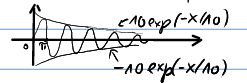
\includegraphics[width=4 cm,height=2cm]{bsp kap 21.31.1}
	\end{figure}\\ 
	\underline{Bsp.:} $y(x)=exp(\frac{x}{10}\sin x)$ aufschaukelnde Schwingung mit $\alpha \textgreater0$\\
	\begin{figure}[h]
		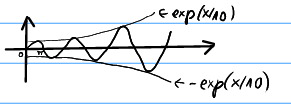
\includegraphics[width=4 cm,height=2cm]{bsp kap 21.31.2}
	\end{figure}\\ 
	\\
	\textbf{21.32. \underline{Lösung der inhomogenen DGL}}\\
	Aus der \oraul{Linearität von $\varphi(D)$} folgt das\\
	\\
	\textbf{21.33. \redul{Superpositionsprinzip:}} Ist \greenul{$f=f_1+f_2$} und \greenul{$u_j$ Lsg. von $\varphi(D)u_j=f_j$}, j=1,2, \\
	so liefert \greenul{$u:=u_1+u_2$ eine Lsg.} von \greenul{$\varphi(D)u=f$}.\blackcircle{*}\\
	Strategie: Suche Lsgn. für die einzelnen Summanden von f.\\
	\\
	\textbf{21.34. \underline{Satz:}} \underline{Vor.:} \greenul{$Q\in \mathbb{C}[x], deg\ Q=s \in \mathbb{N}_0, \alpha \in \mathbb{C}$}.\\
	Beh.: Zur \greenul{Inhomogenität $f:=e^{\alpha x}Q$ ex. eine Lsg. von $\blackcircle{*}$ der Gestalt $ee^{\alpha x}R$} mit einem \greenul{$R\in\mathbb{C}[x]$}, wo \greenul{$deg\ R\leq s$ für $\varphi(\alpha)\neq0$}, und \greenul{$deg\ R\leq r+s$ für Nst. $\alpha$ der Ordnung r.}\\
	Beweis siehe \blueul{[Beuser, Satz 16.5.]}\\
	\\
	Nützlich zum Auffinden einer partikulären Lösung von \blackcircle{*}:\\
	\textbf{21.35. \underline{Bem.:}} Ist $P \in \mathbb{C}[x]$, \greenul{$ddeg\ P\leq k$}$\infty\mathbb{N}_0$, so gilt \greenul{$\forall\alpha\in\mathbb{C}\backslash\{0\}:$}\\
		\greenul{$(D-\alpha)^{-1}P=-\frac{1}{\alpha}\sum_{l=0}^{k}\frac{1}{\alpha^l}D^lP$}.\\
		\underline{Bew.:} \oraul{$(D-\alpha)\cdot$ r.S.}=$\underbrace{-\frac{1}{\alpha}\sum_{l=0}^{k}\frac{1}{\alpha^l}D^lP}_{=-\sum_{l=1}^{k}\frac{1}{\alpha^l}D^lP}+\sum_{l=0}^{k}\frac{1}{\alpha^l}D^lP=\frac{1}{\alpha^0}D^0P=$\oraul{P=$(D-\alpha)\cdot$l.S.}\checkmark\\
		\strut\hfill$\square$\\
	\textbf{21.36. \underline{Bsp.:}} \fcolorbox{red}{white}{$y''-4y'+4y=x^2$}.\\
	Die l.S. ist ($D^2-4D+4$)y=$(D-2)^2y$, nach \blueul{21.14.(b)} und \blueul{21.21.(d)} liefern \greenul{$e^{2x},xe^{2x}$ ein Fundamentalsystem der homogenen DGL.}\\
	Mit \blueul{21.35.} erhält man eine \greenul{partikuläre Lsg. y} durch \greenul{$((D-\alpha)^{-1})^2$. l.S.}\\
	=$((D-\alpha)^{-1})^2x^2=(-\frac{1}{2}(1+\frac{1}{2}D+\frac{1}{4}D^2))^2x^2=\frac{1}{4}(1+D+\frac{3}{4}D^2)x^2=$\greenul{$\frac{1}{4}(x^2)+2x+\frac{3}{2}$}.\\
	\textopencorner$(1+\frac{1}{2}D+\frac{1}{4}D^2)^2=1+2D+(\frac{1}{2}D)^2+\frac{1}{4}D^2$+ terme mit $D^h, \ h\geq 3$\textcorner\\ 
	\textbf{21.37. \underline{Standardbsp. der Physik:}} Frei schwingendes Federpendel in der Mechanik\\
	$\blackcircle{*}$ \fcolorbox{red}{white}{m $\overset{\cdot\cdot}{y}+r\dot{y}+ky=0$}, y Auslenkung, Variable: Zeit t$\geq$0, m$\textgreater$0 Masse, r$\geq$0 Reibung, k\textgreater0 Federkonstante\\
	$\rightarrow a=\frac{r}{m},\ b=\frac{k}{m}$ von der Form $\blackcircle{*}_h$\\
	\\
	\textbf{21.38. \underline{Standardbsp. der Physik:}} geschlossener Schwingkreis in der Elektrotechnik \\
	\fcolorbox{red}{white}{$CL\overset{\cdot \cdot}{y}+CR\dot{y}+y=0$}, y Kondensatorladung, Variable: Zeit $t\geq0$ C Kapazität, R Widerstand,\\
	$\rightarrow=\frac{R}{L},\ b=\frac{1}{CL}$ von der Form $\blackcircle{*}_h$, genauso! L Induktivität\\
	\textopencorner Standardbsp. in Wirtschaftstheorie: Konjunkturschwankungen \textcorner\\
	\\
	\underline{Lsg., nur im Fall Federpendel}\blueul{21.37:}\\
	\textbf{21.39. (a):} \redul{Harmonische Oszillator/harmonische Schwingung} \underline{im Fall r=0} (ohne Reibung)\\
	Mit \yelul{$w_0$}:=$\sqrt{\frac{k}{m}}$ wird \blackcircle{*} in der Form \redul{$\overset{\cdot \cdot }{y}+w_0^2y=0$} notiert.\\
	$\rightarrow$\greenul{$\varphi(\lambda)=\lambda^2+w_0^2=(\lambda-iw_0)(\lambda+iw_o),\ y(t)=c_1\sin(w_0t)+c_2\cos(w_0t), \ c_1,c_2\in \mathbb{R}$}\\
	Mit $A\geq 0,\ \beta \in \mathbb{R}$ geeignet schreibe dies als \greenul{$y(t)=A\sin(w_0t+\beta)$}, \redul{A:Amplitude, $w_0$: Eigenfrequenz}.\\
	\\
	\textbf{21.40. (b):} \underline{Für $r\textgreater0$} setzen \yelul{$\sigma$}:= $\frac{r}{2m}=\frac{a}{2}\rightarrow$\greenul{$a^2-4b$}=$\frac{r^2}{m^2}-4\frac{k}{m}=$\greenul{$4(\sigma^2-w_0^2)$}.\\
	\underline{1. Fall:} \redul{$a^2-4b\textgreater0\Leftrightarrow \sigma\textgreater w_0$}.\\
	Dann: $\lambda_{1,2}=\frac{1}{2}(-a\pm\sqrt{a^2-4b})=-\sigma\pm\sqrt{\sigma^2-w_0^2},$\\
	$\rightarrow$ \greenul{$y(t)=e^{-\sigma t}(c_1e^{\sqrt{\sigma^2-w_0^2}t}+c_2e^{-\sqrt{\sigma^2-w_0^2}t})$}\\
	Da \greenul{$-\sigma\pm\sqrt{\sigma^2-w_0^2}\textless 0$}: \redul{abklingende Kriechbewegung/aperiodischer Fall/starke Dämpfung} \textopencorner in \blueul{21.36.:} Entladung des Kondensators\textcorner\\
	\\
	\textbf{21.41. \redul{periodische Störung:}} \redul{$\overset{\cdot \cdot}{y}+a\dot{y}+by=\overset{\cdot \cdot}{y}+2\sigma \dot{y}+w_0^2y= A\cos(wt) \textbf{ bzw. }A exp(iwt)$}\\
	mit \redul{Störamplitude A \textgreater 0, Störfrequenz $w_0\textgreater 0$}\\
	Setze \yelul{$\gamma:=$}$\frac{A}{\varphi(iw)}=\frac{A}{w_0^2-w^2+i2\sigma w}=:$ \redul{$|\gamma|\exp(i\sigma)$}\\
	\greenul{Partikuläre Lsg: z(t)=$|\gamma| \exp(i(wt-\sigma))$}, $|\gamma|:$\redul{Amplitude, $\sigma$: Phasenverschiebung}.\\
	Im Fall \redul{$w_0^2-2\sigma^2\leq0$}$\Leftrightarrow w_0\geq\sqrt{2}\sigma$ der \redul{"schwache Dämpfung"} erhält man das \redul{strikte Min.} \underline{für $w^*$}:= $\sqrt{w_0^2-2\sigma^2}\rightarrow|\gamma(w^*)|=\frac{A}{2\sigma\sqrt{w_0^2-\sigma^2}}$\\
	$w^*$ heißt \redul{Resonanzfrequenz} \textopencorner $|\gamma|$ maximal $\Leftrightarrow$ $w^*$ minimal \textcorner\\
	Weiter: $\sigma \rightarrow$0 $\Rightarrow\ w^*\rightarrow w_0,$ \greenul{$|\gamma(w^*)|\rightarrow\infty$}\\
	\underline{Falls}\redul{$w=w_0$}: $\overset{\cdot \cdot}{z}+w_02 z=A\exp(iw_0t)\rightarrow$ Lsg. \greenul{$\frac{A}{2iw_0} t \exp(iw_0t)$},\\
	reell: \greenul{$y^*(t)=\frac{A}{2w_0}t\sin(w_0t)\xrightarrow{t\rightarrow\infty}\infty$} \redul{Resonanzkatastrophe}\\
	\underline{Falls} \redul{$w\neq w_0$}: " hat Lsg. \greenul{$\frac{A}{w^2-w_0^2}\exp(iwt)$}\\
	\underline{Falls} \redul{$w_0^2-2\sigma^2\textless0$} $\Leftrightarrow w_0\textless\sqrt{2}\sigma$ \redul{"starke Dämpfung"}: \greenul{Max. von $|\gamma(w)|$ für $w^*=0$} mit \greenul{$|\gamma(0)|=\frac{A}{q_0^2}$}, und \greenul{$|\gamma(w)|\xrightarrow{w\rightarrow\infty}0$}.
\end{document}